\section{Ensemble}
A number of different strategies for combining the ensemble members will be described in this section. This includes averaging and weighted averaging the detections. The method for inferring each of the ensemble will be the same apart from the combination set. This is shown in \figref{ensemble_ex}. Firstly, for a object proposal in an image found with the \gls{rpn} each network will infer a bounding box and associated confidence for all classes. After this the given ensemble combination method determines the final detection. 

\subsection{Weighted Average Ensemble}
Each of then 10 trained networks will be used on all object proposals found using the \gls{rpn}. Weights will be distributed evenly across each of the five different types of factors. The weighted average ensemble is determined for each bounding-box and the associated confidence by:

\begin{equation}
	E_{j} = \frac{1}{n} \sum_{i=1}^{n} w_ip_{i,j} 
\end{equation}

where $n$ is the number of detections found by the $n$ networks, $w_i$ is the weight associated with the i-th ensemble factor and $p$ is the detection value to be averaged. Finally, $j$ is one of the five values found by each detection, namely the four corners of the bounding-box and the associated confidence.
Weights are determined in pairs for each of the 5 ensemble factors, where the total sum of weights is equal to $n$. If each detection were to be weighted equally all $w$ would be equal to 1. As the weights are calculated in pairs each ensemble factor is overall weighted equally as the pair of weights can at most be equal to 2. By using this tactic in between the two sets of network for a given factor can be weighted differently but overall each factor is weighted equally.
Weights for a given factor is found according to where the the test image lies for that factors training distribution data. For example, the subsets of training data for Gaussian blur was determined according to the line shown in \figref{blur_dist}. 

\add[inline]{line showing split in training data}

\begin{figure}[H]
  \centering
    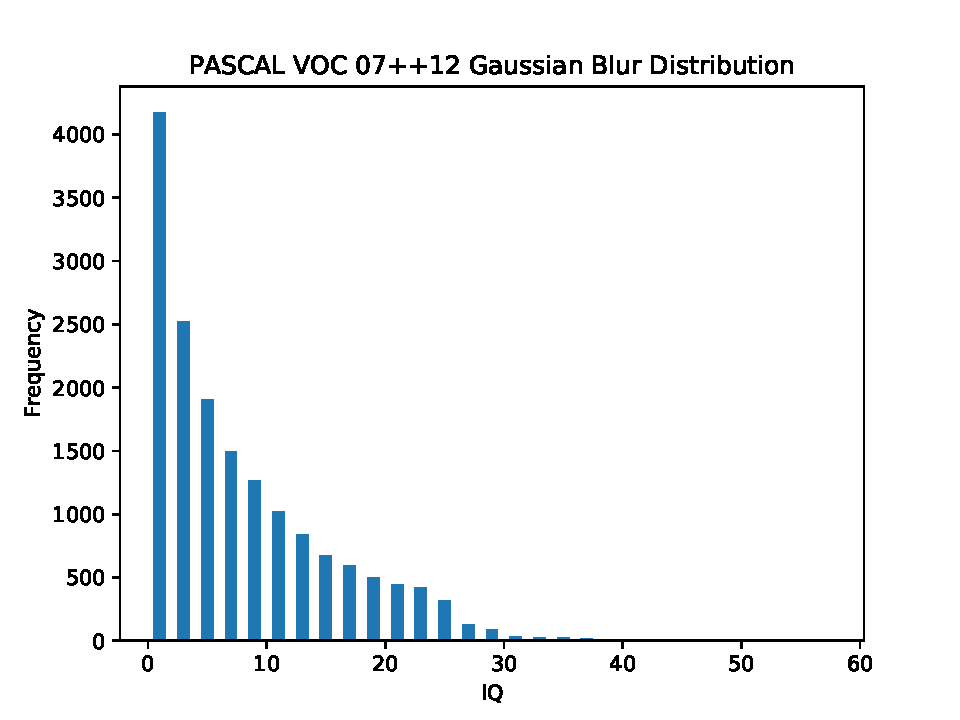
\includegraphics[width=0.8\textwidth]{Figs/Implementation/GaussianBlurdist.pdf}
      \caption{}
    \label{fig:blur_dist}
\end{figure}

The quality, $q_i$ with respect to blur for a given image is determined using the appropriate Deep IQA model, if the quality is below the value used to split the data the weights are calculated for the detection found with the given lower network by:

\begin{equation}
	w_{Lower} = 2 - \frac{split - q_i}{split - minq_i}
\end{equation}

and the weight for the upper network $w_{Upper}$ by:

\begin{equation}
	w_{Upper} = 2 - w_{Lower}
\end{equation}

where $split$ is the value used to split the training data and $minq_i$ is the minimum quality for the given factor in the training set.

However, if the quality is above $split$ the $w_{Upper}$ is calculated by:

\begin{equation}
	w_{Upper} = 2 - \frac{maxq_i - q_i}{maxq_i - split}
\end{equation}

and lower weight $w_{Lower}$:

\begin{equation}
	w_{Lower} = 2 - w_{Upper}.
\end{equation}

\subsubsections{Results}
\begin{comment}
AP for aeroplane = 0.2492
AP for bicycle = 0.3045
AP for bird = 0.2650
AP for boat = 0.2639
AP for bottle = 0.2409
AP for bus = 0.2693
AP for car = 0.2630
AP for cat = 0.3153
AP for chair = 0.2175
AP for cow = 0.2320
AP for diningtable = 0.3623
AP for dog = 0.2826
AP for horse = 0.3163
AP for motorbike = 0.2991
AP for person = 0.3278
AP for pottedplant = 0.2012
AP for sheep = 0.2438
AP for sofa = 0.2620
AP for train = 0.3121
AP for tvmonitor = 0.2691
Mean AP = 0.2748
~~~~~~~~
Results:
0.249
0.304
0.265
0.264
0.241
0.269
0.263
0.315
0.218
0.232
0.362
0.283
0.316
0.299
0.328
0.201
0.244
0.262
0.312
0.269
0.275
~~~~~~~~
\end{comment}

